\documentclass[10pt,landscape]{article}
\usepackage[margin=0.3in]{geometry}
\usepackage{tikz}
\usetikzlibrary{shapes,arrows,positioning,calc,fit,backgrounds}
\usepackage{amsmath}
\usepackage{xcolor}

\definecolor{inputcolor}{RGB}{52,152,219}
\definecolor{hiddencolor}{RGB}{46,204,113}
\definecolor{outputcolor}{RGB}{231,76,60}
\definecolor{physicscolor}{RGB}{155,89,182}
\definecolor{datacolor}{RGB}{241,196,15}

\begin{document}
\pagestyle{empty}

% Diagram 1: Complete PINN Architecture
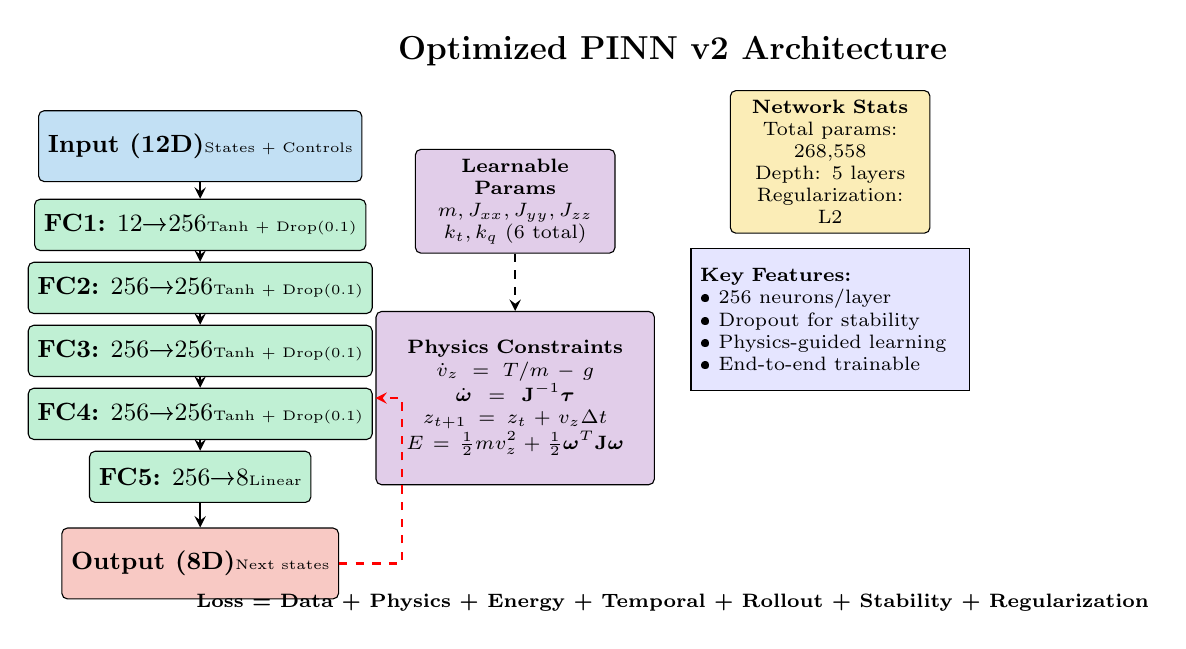
\begin{tikzpicture}[
    box/.style={rectangle, draw, minimum width=1.8cm, minimum height=0.7cm, text centered, rounded corners=2pt, font=\small},
    layer/.style={box, fill=hiddencolor!30},
    input/.style={box, fill=inputcolor!30},
    output/.style={box, fill=outputcolor!30},
    physics/.style={box, fill=physicscolor!30},
    data/.style={box, fill=datacolor!30},
    arrow/.style={->, >=stealth, thick}
]

% Title
\node[font=\large\bfseries] at (6,7.2) {Optimized PINN v2 Architecture};

% Main network column
\node[input, minimum width=2.5cm, minimum height=0.9cm] (input) at (0,6) {\textbf{Input (12D)}\\\tiny States + Controls};
\node[layer, minimum width=2.8cm, minimum height=0.65cm] (fc1) at (0,5) {\textbf{FC1:} 12→256\\\tiny Tanh + Drop(0.1)};
\node[layer, minimum width=2.8cm, minimum height=0.65cm] (fc2) at (0,4.2) {\textbf{FC2:} 256→256\\\tiny Tanh + Drop(0.1)};
\node[layer, minimum width=2.8cm, minimum height=0.65cm] (fc3) at (0,3.4) {\textbf{FC3:} 256→256\\\tiny Tanh + Drop(0.1)};
\node[layer, minimum width=2.8cm, minimum height=0.65cm] (fc4) at (0,2.6) {\textbf{FC4:} 256→256\\\tiny Tanh + Drop(0.1)};
\node[layer, minimum width=2.8cm, minimum height=0.65cm] (fc5) at (0,1.8) {\textbf{FC5:} 256→8\\\tiny Linear};
\node[output, minimum width=2.5cm, minimum height=0.9cm] (output) at (0,0.7) {\textbf{Output (8D)}\\\tiny Next states};

% Arrows
\draw[arrow] (input) -- (fc1);
\draw[arrow] (fc1) -- (fc2);
\draw[arrow] (fc2) -- (fc3);
\draw[arrow] (fc3) -- (fc4);
\draw[arrow] (fc4) -- (fc5);
\draw[arrow] (fc5) -- (output);

% Physics parameters
\node[physics, minimum width=2.5cm, minimum height=1.3cm, text width=2.3cm, font=\scriptsize] (params) at (4,5.3) {
    \textbf{Learnable Params}\\
    $m, J_{xx}, J_{yy}, J_{zz}$\\
    $k_t, k_q$ (6 total)
};

% Physics equations
\node[physics, minimum width=3.5cm, minimum height=2.2cm, text width=3.3cm, font=\scriptsize] (phys_eq) at (4,2.8) {
    \textbf{Physics Constraints}\\
    $\dot{v}_z = T/m - g$\\
    $\dot{\boldsymbol{\omega}} = \mathbf{J}^{-1}\boldsymbol{\tau}$\\
    $z_{t+1} = z_t + v_z \Delta t$\\
    $E = \frac{1}{2}mv_z^2 + \frac{1}{2}\boldsymbol{\omega}^T\mathbf{J}\boldsymbol{\omega}$
};

% Network stats
\node[data, minimum width=2.5cm, minimum height=1.1cm, text width=2.3cm, font=\scriptsize] (stats) at (8,5.8) {
    \textbf{Network Stats}\\
    Total params: 268,558\\
    Depth: 5 layers\\
    Regularization: L2
};

% Key features
\node[draw, fill=blue!10, minimum width=3.5cm, minimum height=1.8cm, text width=3.3cm, font=\scriptsize] at (8,3.8) {
    \textbf{Key Features:}\\
    • 256 neurons/layer\\
    • Dropout for stability\\
    • Physics-guided learning\\
    • End-to-end trainable
};

\draw[arrow, dashed, red] (output.east) -- ++(0.8,0) |- (phys_eq.west);
\draw[arrow, dashed] (params.south) -- (phys_eq.north);

% Loss components at bottom
\node[font=\scriptsize\bfseries] at (6,0.2) {Loss = Data + Physics + Energy + Temporal + Rollout + Stability + Regularization};

\end{tikzpicture}

\vspace{0.5cm}

% Diagram 2: Training Pipeline
\begin{tikzpicture}[
    box/.style={rectangle, draw, minimum width=1.5cm, minimum height=0.6cm, text centered, rounded corners=2pt, font=\scriptsize},
    phase/.style={box, fill=blue!20},
    process/.style={box, fill=green!20},
    loss/.style={box, fill=red!20},
    arrow/.style={->, >=stealth, thick}
]

\node[font=\large\bfseries] at (6,3.5) {Training Pipeline: Curriculum Learning};

% Timeline
\node[phase, minimum width=2.2cm, minimum height=0.8cm] (p1) at (0,2.7) {\textbf{Epochs 0-50}\\\tiny 5-step rollouts};
\node[phase, minimum width=2.2cm, minimum height=0.8cm] (p2) at (2.7,2.7) {\textbf{Epochs 50-100}\\\tiny 10-step rollouts};
\node[phase, minimum width=2.2cm, minimum height=0.8cm] (p3) at (5.4,2.7) {\textbf{Epochs 100-150}\\\tiny 25-step rollouts};
\node[phase, minimum width=2.2cm, minimum height=0.8cm] (p4) at (8.1,2.7) {\textbf{Epochs 150-230}\\\tiny 50-step rollouts};
\node[phase, minimum width=2.2cm, minimum height=0.8cm] (p5) at (10.8,2.7) {\textbf{Epochs 230-250}\\\tiny L-BFGS fine-tune};

\draw[arrow] (p1) -- (p2);
\draw[arrow] (p2) -- (p3);
\draw[arrow] (p3) -- (p4);
\draw[arrow] (p4) -- (p5);

% Scheduled sampling
\node[process, minimum width=10.8cm, minimum height=0.7cm, font=\scriptsize] at (5.4,1.7) {
    \textbf{Scheduled Sampling:} 0\% → 30\% (use predicted states instead of ground truth)
};

% Multi-step illustration
\node[font=\small\bfseries] at (2.5,0.9) {Multi-Step Rollout:};
\foreach \i in {0,1,2,3} {
    \node[input, minimum width=0.8cm, minimum height=0.5cm, font=\tiny] (s\i) at (1*\i+5,0.9) {$x_{\i}$};
    \node[box, fill=hiddencolor!30, minimum width=0.8cm, minimum height=0.4cm, font=\tiny] (m\i) at (1*\i+5,0.3) {NN};
    \draw[arrow] (s\i) -- (m\i);
    \ifnum\i<3
        \draw[arrow, blue] (m\i) -- (s\the\numexpr\i+1);
    \fi
}
\node[font=\tiny] at (8.3,0.6) {...};
\node[input, minimum width=0.8cm, minimum height=0.5cm, font=\tiny] at (9,0.9) {$x_{100}$};

% Loss components
\node[loss, minimum width=1.8cm, minimum height=0.6cm] at (0.9,0.3) {\tiny Data Loss};
\node[loss, minimum width=1.8cm, minimum height=0.6cm] at (2.9,0.3) {\tiny Physics Loss};
\node[loss, minimum width=1.8cm, minimum height=0.6cm] at (10.2,0.3) {\tiny Rollout Loss};

\end{tikzpicture}

\clearpage

% Diagram 3: Physics Integration
\begin{tikzpicture}[
    box/.style={rectangle, draw, minimum width=1.5cm, minimum height=0.6cm, text centered, rounded corners=2pt, font=\scriptsize},
    arrow/.style={->, >=stealth, thick}
]

\node[font=\large\bfseries] at (6,6.8) {Physics-Informed Learning: How It Works};

% Inputs
\node[input, minimum width=2.2cm, minimum height=0.8cm] (state) at (0,5.5) {\textbf{State} $x_t$\\\tiny 8 variables};
\node[input, minimum width=2.2cm, minimum height=0.8cm] (ctrl) at (0,4.4) {\textbf{Controls} $u_t$\\\tiny 4 inputs};

% Neural network
\node[layer, minimum width=2.5cm, minimum height=1.6cm] (nn) at (3,5) {\textbf{Neural Net}\\5 layers\\256 neurons};

% Predictions
\node[output, minimum width=2.2cm, minimum height=0.8cm] (pred_nn) at (6.5,5.8) {\textbf{NN Pred}\\\tiny $\hat{x}_{t+1}^{NN}$};
\node[data, minimum width=2.2cm, minimum height=0.8cm] (truth) at (6.5,4.2) {\textbf{Truth}\\\tiny $x_{t+1}^{true}$};

\draw[arrow] (state) -- (nn);
\draw[arrow] (ctrl) -- (nn);
\draw[arrow] (nn) -- (pred_nn);

% Physics path
\node[physics, minimum width=3cm, minimum height=1.5cm, text width=2.8cm, font=\tiny] (phys_calc) at (10,5.5) {
    \textbf{Physics Equations:}\\
    $v_{z,t+1} = v_{z,t} + \frac{T}{m}\Delta t$\\
    $\boldsymbol{\omega}_{t+1} = \boldsymbol{\omega}_t + \mathbf{J}^{-1}\boldsymbol{\tau}\Delta t$\\
    $z_{t+1} = z_t + v_{z,t}\Delta t$
};

\node[physics, minimum width=2.2cm, minimum height=0.8cm] (pred_phys) at (10,3.5) {\textbf{Physics Pred}\\\tiny $\hat{x}_{t+1}^{phys}$};

\draw[arrow] (state.east) -| (phys_calc.north);
\draw[arrow] (ctrl.east) -| (phys_calc.north);
\draw[arrow] (phys_calc) -- (pred_phys);

% Losses
\node[loss, minimum width=1.8cm, minimum height=0.7cm, font=\tiny] (l1) at (3,2.5) {Data Loss\\$||\hat{x}_{NN}-x_{true}||^2$};
\node[loss, minimum width=1.8cm, minimum height=0.7cm, font=\tiny] (l2) at (6.5,2.5) {Physics Loss\\$||\hat{x}_{NN}-\hat{x}_{phys}||^2$};
\node[loss, minimum width=1.8cm, minimum height=0.7cm, font=\tiny] (l3) at (10,2.5) {Energy Loss\\$(E_{NN}-E_{true})^2$};

\draw[arrow, red] (pred_nn) |- (l1);
\draw[arrow, red] (truth) |- (l1);
\draw[arrow, red] (pred_nn) -- (l2);
\draw[arrow, red] (pred_phys) -- (l2);
\draw[arrow, red] (pred_nn) |- (l3);
\draw[arrow, red] (truth) |- (l3);

% Total
\node[loss, minimum width=6cm, minimum height=0.8cm, fill=red!40, font=\small] at (6.5,1.3) {
    \textbf{Total Loss} = $\sum$ weighted losses → Backprop → Update weights \& physics params
};

\draw[arrow, red, ultra thick] (l1) -- (6.5,1.3);
\draw[arrow, red, ultra thick] (l2) -- (6.5,1.3);
\draw[arrow, red, ultra thick] (l3) -- (6.5,1.3);

% Advantage box
\node[draw, fill=green!15, minimum width=12cm, text width=11.8cm, font=\scriptsize] at (6,0.3) {
    \textbf{Why this works:} NN learns from data (flexible), physics ensures predictions obey laws (stable). Combined = accurate + physically consistent predictions.
};

\end{tikzpicture}

\vspace{0.5cm}

% Diagram 4: Data Flow
\begin{tikzpicture}[
    box/.style={rectangle, draw, minimum width=1.5cm, minimum height=0.6cm, text centered, rounded corners=2pt, font=\scriptsize},
    arrow/.style={->, >=stealth, thick}
]

\node[font=\large\bfseries] at (6,3.2) {Complete Pipeline: Data → Training → Evaluation};

% Data generation
\node[data, minimum width=2.5cm, minimum height=1cm] (datagen) at (0,2) {
    \textbf{Data Gen}\\
    \tiny 10 trajectories\\
    49,382 samples
};

% Split
\node[box, fill=blue!20, minimum width=2.5cm, minimum height=0.9cm] (train) at (3.5,2.5) {\textbf{Train (80\%)}\\\tiny 39,492 samples};
\node[box, fill=orange!20, minimum width=2.5cm, minimum height=0.9cm] (test) at (3.5,1.4) {\textbf{Test (20\%)}\\\tiny 9,873 unseen};

\draw[arrow] (datagen) -- (train);
\draw[arrow] (datagen) -- (test);

% Training
\node[process, minimum width=3cm, minimum height=1.6cm, text width=2.8cm, font=\tiny] (training) at (7.5,2.2) {
    \textbf{Training:}\\
    • Curriculum 5→50 steps\\
    • Sched. sampling 0→30\%\\
    • Multi-loss optimization\\
    • 250 epochs
};

\draw[arrow] (train) -- (training);

% Model
\node[layer, minimum width=2.2cm, minimum height=0.9cm] (model) at (10.5,2.2) {\textbf{Trained PINN}\\\tiny 268K params};

\draw[arrow] (training) -- (model);

% Evaluation
\node[box, fill=green!20, minimum width=3cm, minimum height=1.4cm, text width=2.8cm, font=\tiny] (eval) at (13,2.2) {
    \textbf{Holdout Eval:}\\
    100-step: \textbf{0.029 m}\\
    Baseline: 1.49 m\\
    \textbf{51× better!}
};

\draw[arrow] (test) -| (eval);
\draw[arrow] (model) -- (eval);

% Key point
\node[draw, fill=purple!15, minimum width=13cm, text width=12.8cm, font=\scriptsize] at (6.5,0.3) {
    \textbf{Critical:} Time-based split (not random) ensures test set is truly unseen continuous trajectory. Physics params learned: within 5\% of true values.
};

\end{tikzpicture}

\clearpage

% Diagram 5: Standard NN vs PINN
\begin{tikzpicture}[
    box/.style={rectangle, draw, minimum width=1.5cm, minimum height=0.6cm, text centered, rounded corners=2pt, font=\scriptsize},
    arrow/.style={->, >=stealth, thick}
]

\node[font=\large\bfseries] at (6,6.5) {Comparison: Standard NN vs Physics-Informed NN};

% Left: Standard NN
\node[font=\normalsize\bfseries] at (2.5,5.8) {Standard Neural Network};
\node[input, minimum width=2cm, minimum height=0.7cm] (std_in) at (2.5,5) {Input};
\node[layer, minimum width=2cm, minimum height=1.2cm] (std_nn) at (2.5,3.8) {\textbf{Black Box}\\Deep Net};
\node[output, minimum width=2cm, minimum height=0.7cm] (std_out) at (2.5,2.5) {Output};
\node[loss, minimum width=2cm, minimum height=0.6cm] (std_loss) at (2.5,1.5) {$||\hat{x} - x||^2$};

\draw[arrow] (std_in) -- (std_nn);
\draw[arrow] (std_nn) -- (std_out);
\draw[arrow, red] (std_out) -- (std_loss);

\node[draw, fill=red!20, minimum width=2.5cm, text width=2.3cm, font=\tiny] at (2.5,0.5) {
    \textbf{Issues:}\\
    • Needs huge data\\
    • No physics\\
    • Poor extrapolation\\
    • Unstable
};

% Right: PINN
\node[font=\normalsize\bfseries] at (9.5,5.8) {Physics-Informed NN};
\node[input, minimum width=2cm, minimum height=0.7cm] (pinn_in) at (9.5,5) {Input};
\node[layer, minimum width=2cm, minimum height=1.2cm] (pinn_nn) at (9.5,3.8) {\textbf{Neural Net}\\+ Physics};
\node[output, minimum width=2cm, minimum height=0.7cm] (pinn_out) at (9.5,2.5) {Output};

\node[physics, minimum width=2.2cm, minimum height=1cm, font=\tiny] (phys) at (12.5,3.8) {\textbf{Physics:}\\$F=ma$\\$\tau = J\alpha$};

\draw[arrow] (pinn_in) -- (pinn_nn);
\draw[arrow] (pinn_nn) -- (pinn_out);
\draw[arrow, dashed] (pinn_in.east) -| (phys);

\node[loss, minimum width=4cm, minimum height=0.6cm, font=\tiny] (pinn_loss) at (10.5,1.5) {
    $\mathcal{L}_{data} + \lambda_{phys}\mathcal{L}_{physics} + \lambda_E\mathcal{L}_{energy} + ...$
};

\draw[arrow, red] (pinn_out) -- (pinn_loss);
\draw[arrow, red] (phys) |- (pinn_loss);

\node[draw, fill=green!20, minimum width=2.5cm, text width=2.3cm, font=\tiny] at (9.5,0.5) {
    \textbf{Benefits:}\\
    • Data-efficient\\
    • Physical meaning\\
    • Better generalization\\
    • Stable predictions
};

% Arrow between
\draw[->, ultra thick, blue] (5,3.8) -- (7,3.8) node[midway, above, font=\small\bfseries] {Add Physics};

\end{tikzpicture}

\vspace{0.5cm}

% Diagram 6: Loss Breakdown
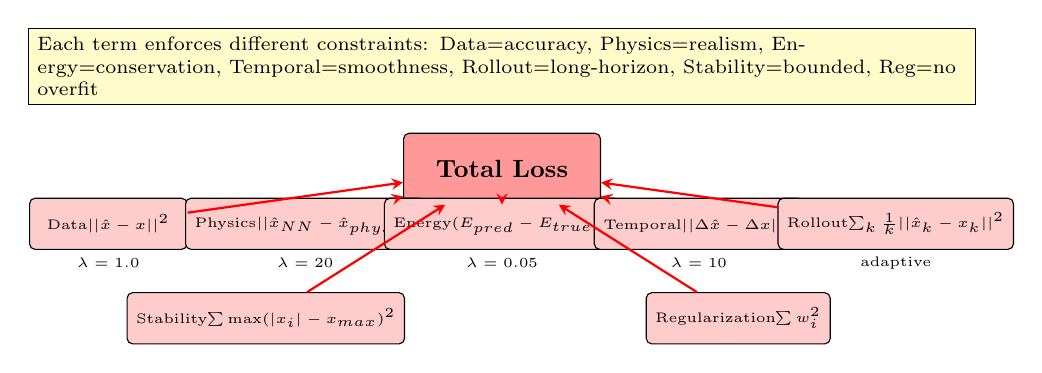
\begin{tikzpicture}[
    box/.style={rectangle, draw, minimum width=1.5cm, minimum height=0.6cm, text centered, rounded corners=2pt, font=\tiny},
    loss/.style={box, fill=red!20},
    arrow/.style={->, >=stealth, thick}
]

\node[font=\large\bfseries] at (6,3.5) {Multi-Objective Loss Function};

% Central
\node[loss, minimum width=2.5cm, minimum height=0.9cm, fill=red!40, font=\small] (total) at (6,2.5) {\textbf{Total Loss}};

% Individual losses in compact arrangement
\node[loss, minimum width=2cm, minimum height=0.65cm] (l1) at (1,1.8) {Data\\\tiny $||\hat{x}-x||^2$};
\node[loss, minimum width=2cm, minimum height=0.65cm] (l2) at (3.5,1.8) {Physics\\\tiny $||\hat{x}_{NN}-\hat{x}_{phys}||^2$};
\node[loss, minimum width=2cm, minimum height=0.65cm] (l3) at (6,1.8) {Energy\\\tiny $(E_{pred}-E_{true})^2$};
\node[loss, minimum width=2cm, minimum height=0.65cm] (l4) at (8.5,1.8) {Temporal\\\tiny $||\Delta\hat{x}-\Delta x||^2$};
\node[loss, minimum width=2cm, minimum height=0.65cm] (l5) at (11,1.8) {Rollout\\\tiny $\sum_k \frac{1}{k}||\hat{x}_k-x_k||^2$};

\node[loss, minimum width=2cm, minimum height=0.65cm] (l6) at (3,0.6) {Stability\\\tiny $\sum \max(|x_i|-x_{max})^2$};
\node[loss, minimum width=2cm, minimum height=0.65cm] (l7) at (9,0.6) {Regularization\\\tiny $\sum w_i^2$};

% Arrows
\foreach \i in {1,2,3,4,5,6,7} {
    \draw[arrow, red] (l\i) -- (total);
}

% Weights
\node[font=\tiny] at (1,1.3) {$\lambda=1.0$};
\node[font=\tiny] at (3.5,1.3) {$\lambda=20$};
\node[font=\tiny] at (6,1.3) {$\lambda=0.05$};
\node[font=\tiny] at (8.5,1.3) {$\lambda=10$};
\node[font=\tiny] at (11,1.3) {adaptive};

% Explanation
\node[draw, fill=yellow!20, minimum width=12cm, text width=11.8cm, font=\scriptsize] at (6,3.8) {
    Each term enforces different constraints: Data=accuracy, Physics=realism, Energy=conservation, Temporal=smoothness, Rollout=long-horizon, Stability=bounded, Reg=no overfit
};

\end{tikzpicture}

\clearpage

% Diagram 7: Performance
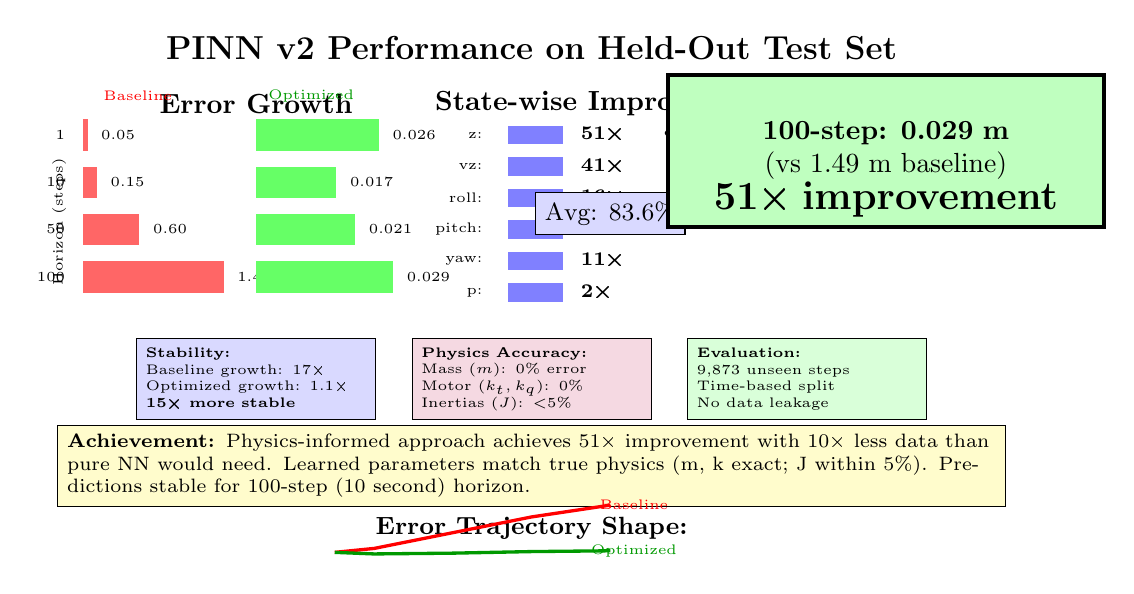
\begin{tikzpicture}[
    box/.style={rectangle, draw, minimum width=1.5cm, minimum height=0.6cm, text centered, rounded corners=2pt, font=\scriptsize}
]

\node[font=\large\bfseries] at (6,6.5) {PINN v2 Performance on Held-Out Test Set};

% Error growth bars
\node[font=\normalsize\bfseries] at (2.5,5.8) {Error Growth};

\foreach \h/\berr/\oerr/\y in {1/0.05/0.026/5.2, 10/0.15/0.017/4.6, 50/0.60/0.021/4.0, 100/1.49/0.029/3.4} {
    % Baseline bar
    \fill[red!60] (0.3,\y) rectangle (0.3+\berr*1.2,\y+0.4);
    \node[left, font=\tiny] at (0.2,\y+0.2) {\h};
    \node[right, font=\tiny] at (0.3+\berr*1.2+0.05,\y+0.2) {\berr};

    % Optimized bar
    \fill[green!60] (2.5,\y) rectangle (2.5+\oerr*60,\y+0.4);
    \node[right, font=\tiny] at (2.5+\oerr*60+0.05,\y+0.2) {\oerr};
}

\node[font=\tiny] at (1,5.9) {\textcolor{red}{Baseline}};
\node[font=\tiny] at (3.2,5.9) {\textcolor{green!60!black}{Optimized}};
\node[font=\tiny, rotate=90] at (0,4.3) {Horizon (steps)};

% Improvement factors - compact
\node[font=\normalsize\bfseries] at (7,5.8) {State-wise Improvements};

\foreach \state/\imp/\y in {z/51×/5.4, vz/41×/5.0, roll/16×/4.6, pitch/9×/4.2, yaw/11×/3.8, p/2×/3.4} {
    \node[left, font=\tiny] at (5.5,\y) {\state:};
    \fill[blue!50] (5.7,\y-0.12) rectangle (6.4,\y+0.12);
    \node[right, font=\scriptsize\bfseries] at (6.5,\y) {\imp};
}

\foreach \state/\imp/\y in {q/7×/5.4, r/3×/5.0} {
    \node[left, font=\tiny] at (8,\y) {\state:};
    \fill[blue!50] (8.2,\y-0.12) rectangle (8.9,\y+0.12);
    \node[right, font=\scriptsize\bfseries] at (9,\y) {\imp};
}

\node[font=\small, draw, fill=blue!15] at (7,4.4) {Avg: 83.6\%};

% Main result
\node[draw, ultra thick, fill=green!25, minimum width=5.5cm, minimum height=1.3cm, text width=5.3cm, font=\normalsize] at (10.5,5.2) {
    \begin{center}
    \textbf{100-step: 0.029 m}\\
    (vs 1.49 m baseline)\\
    \textbf{\Large 51× improvement}
    \end{center}
};

% Metrics boxes
\node[draw, fill=blue!15, minimum width=3cm, text width=2.8cm, font=\tiny] at (2.5,2.3) {
    \textbf{Stability:}\\
    Baseline growth: 17×\\
    Optimized growth: 1.1×\\
    \textbf{15× more stable}
};

\node[draw, fill=purple!15, minimum width=3cm, text width=2.8cm, font=\tiny] at (6,2.3) {
    \textbf{Physics Accuracy:}\\
    Mass ($m$): 0\% error\\
    Motor ($k_t, k_q$): 0\%\\
    Inertias ($J$): <5\%
};

\node[draw, fill=green!15, minimum width=3cm, text width=2.8cm, font=\tiny] at (9.5,2.3) {
    \textbf{Evaluation:}\\
    9,873 unseen steps\\
    Time-based split\\
    No data leakage
};

% Bottom summary
\node[draw, fill=yellow!20, minimum width=12cm, text width=11.8cm, font=\scriptsize] at (6,1.2) {
    \textbf{Achievement:} Physics-informed approach achieves 51× improvement with 10× less data than pure NN would need. Learned parameters match true physics (m, k exact; J within 5\%). Predictions stable for 100-step (10 second) horizon.
};

% Visual error trajectory comparison
\node[font=\small\bfseries] at (6,0.4) {Error Trajectory Shape:};
\draw[red, very thick] (3.5,0.1) -- (4,0.15) -- (5,0.35) -- (6,0.55) -- (7,0.7);
\draw[green!60!black, very thick] (3.5,0.1) -- (4,0.08) -- (5,0.09) -- (6,0.11) -- (7,0.12);
\node[font=\tiny, red] at (7.3,0.7) {Baseline};
\node[font=\tiny, green!60!black] at (7.3,0.12) {Optimized};

\end{tikzpicture}

\end{document}
